%%%%%%%%%%%%%%%%%%%%%%%%%%%%%%%%%%%%%%%%%%%%%%%%%%%%%%%%%%%%%%%%%%
\section{Quality Assurance}
\label{sec:fdsp-apa-qa}

%\subsection{Component Testing}
%\label{sec:fdsp-apa-qa-testing}

%\fixme{PSL: input needed. are there old tests of APA components we want to present here?  things like the long-term wire tension studies, etc.}  

The most important and complete information for assuring the quality of the \dword{apa} design, components, materials, and construction methods comes from the construction and operation of \dword{pdsp}.  We have learned much about the design and fabrication procedures that has informed the detailed design and plans for the DUNE \dword{apa} construction project. \dword{pdsp} included six full-scale \dword{dune} \dwords{apa} instrumenting two drift regions around a central cathode.  Four of the \dword{pdsp} \dword{apa}s were constructed in the USA at the University of Wisconsin-PSL, and two were made at Daresbury Laboratory in the UK. All were shipped to \dword{cern}, integrated with photon detectors and cold electronics, and tested in a \coldbox prior to installation into the \dword{pdsp} cryostat.  Figure~\ref{fig:sp-apa-pd-photo} shows one of the drift regions in the fully constructed \dword{pdsp} detector.

\begin{dunefigure}[A drift region in ProtoDUNE-SP with installed APAs]{fig:sp-apa-pd-photo}
{One of the two drift regions in the \dword{pdsp} detector at \dword{cern} showing the three installed \dwords{apa} on the left.}
\includegraphics[width=0.9\textwidth]{sp-apa-protodune-photo.jpg}
\end{dunefigure}


\subsection{Results from ProtoDUNE-SP Construction}
\label{sec:fdsp-apa-qa-protodune-const}

A thorough set of \dword{qc} tests were performed and documented throughout the fabrication of the \dword{pdsp} \dword{apa}s.  The positive outcomes give great confidence in the quality of the overall \dword{apa} design  and construction techniques.  Here we summarize some of the testing that was done for \dword{pdsp} and the results.   

%All printed circuit boards (PCBs) were electrically tested and cleaned according to IPC standard. Dimensional checks were performed and all solder pads checked for damage. Any boards that required corrective machining were washed thoroughly, and PCBs were always handled with gloves to prevent contamination.

After each wire layer was applied to an \dword{apa}, electrical continuity between the head and foot boards was checked for each wire.  This test is most useful for the $U$ and $V$ layers, where metal traces on the side boards can be damaged during construction. All boards were visually inspected as construction proceeded.

Channels were also checked for isolation.  In the beginning, wire-to-wire isolation was measured. Those measurements took a lot of time and no problems ever arose.  In the end, each wire was individually hipot tested (a dielectric withstand test) at \SI{1}{kV}. No failures were ever seen. However, leakage currents were seen to be highly dependent on relative humidity.  The surface of the epoxy has some affinity for moisture in the air and provides a measurable leakage path when relative humidity exceeds about \SI{60}{\%}. Tests have confirmed that in a dry environment, such as the liquid argon cryostat, these leakage currents disappear.

Wire tension was measured for all wires at production.  Figure~\ref{fig:sp-apa-pd-tension-prod} displays the measured tensions for wires on the instrumented wire planes ($X, U, V$) for the 6 \dword{pdsp} \dword{apa}s, four constructed at PSL in the US and two at Daresbury Laboratory in the UK.  %The number of wires below and above the tension specification are shown in Table \ref{tab:nwires}. 
In total, \SI{4.4}{\%} of the \num{14972} wires considered for this analysis had a tension below \SI{4}{N} and \SI{22.5}{\%} were above \SI{6}{N}. 
A wire which has a tension higher than specification should not impact the physics in any meaningful way. Wires with tension lower than specification could move slightly out of position and impact detector function primarily through modifying the local electric field. E-field modification can lead to the number of ionization electrons being incorrectly reconstructed in the deconvolution process or alter the transparency so that less than \SI{100}{\%} of the ionization electrons reach the collection plane. Because these processes change the amount of reconstructed charge, they would alter the reconstruction of the energy deposited by charged particles near these wires. A further complication from very low-tension wires might be an increase in noise level, introduced by wire vibrations, which can lead to vortex shedding.  Each of these impacts is expected to be quite small, but to confirm, cosmic muon tracks in \dword{pdsp} data are now being used to test if differences in response can be seen on wires with particularly low tension.  The target tension for \dword{dune} \dword{apa}s has already been increased to \SI{6}{N}, and these \dword{pdsp} studies will quantitatively inform a minimum tension requirement, but no challenges in meeting specifications are foreseen based on current knowledge from \dword{pdsp} construction.   

%The goal of this analysis is to quantify these effects to feed into the design and construction of DUNE.

%\begin{dunetable}[ProtoDUNE-SP APA wire tension plots]{rccccc}{tab:nwires}
%{Total number of wires on each plane for each of the four APAs being considered for this analysis, along with the number and percentage of wires below and above the tension specification of 5 N $\pm$ 1 N.} 
%    Plane & \# Wires & \# Wires $<$ 4 N & $\%$ Wires $<$ 4 N & \# Wires $>$ 6 N & $\%$ Wires $>$ 6 N \\ \toprowrule
%    U     & 4561  & 278 & 6.1 & 1127 & 24.7 \\ \colhline
%    V     & 4552  & 398 & 8.7 & 146  & 3.2  \\ \colhline
%    X     & 1920  & 4   & 0.2 & 115  & 6.0  \\ \colhline
%    Total & 11033 & 680 & 6.2 & 1388 & 12.6 \\ \colhline
%\end{dunetable}

\begin{dunefigure}[ProtoDUNE-SP wire tensions as measured during production]{fig:sp-apa-pd-tension-prod}
{Distributions of wire tensions in the \dword{pdsp} \dword{apa}s for wires longer than \SI{70}{cm}, as measured during production at PSL and Daresbury. For the $X$-plane, every wire has the same length (\SI{598.39}{cm}), and so every wire is included. %The gray lines at \SI{4}{N} and \SI{6}{N} represent the bounds of the 5$\pm$\SI{1}{N} specification used for \dword{pdsp}. 
The histograms for the 6 \dword{apa}s are stacked. %The $X$-plane has few wires which have a tension under specification, while the U and V planes have a total of 680 channels above the 50 cm requirement and a tension under 4 N.
}
\includegraphics[height=0.28\textheight,trim=0mm 0mm 0mm 0mm,clip]{graphics/sp-apa-X-layer-tensions.pdf}
\includegraphics[height=0.28\textheight,trim=0mm 0mm 0mm 0mm,clip]{graphics/sp-apa-V-layer-tensions.pdf}
\includegraphics[height=0.28\textheight,trim=0mm 0mm 0mm 0mm,clip]{graphics/sp-apa-U-layer-tensions.pdf}
\end{dunefigure}

Wire tension measurements were also performed for a subset of wires on each \dword{apa} after arriving at \dword{cern}. Figure~\ref{fig:sp-apa-pd-tension-cern} shows the comparison of tension values measured at \dword{cern} versus at the production site for the selected subset of wires from each wire plane. Based on the traveler documents provided by the production sites, wires having outlier tension values were selected from each \dword{apa} for re-measurement at \dword{cern}. In addition, a set of randomly selected wires from each plane were measured. In total, for six \dword{apa}s, $\sim$1500 wires had their tension re-measured at \dword{cern}. Measurements took place in the clean room with \dword{apa}s hanging vertically, the first time the tensions were sampled in this orientation. Tension measurements were performed by using the laser-photodiode based method, the same as at the production sites. %Some reductions in wire tensions are evident in Figure~\ref{fig:sp-apa-pd-tension-cern}.  %The $X$-plane wire tensions, in particular, are found to be up to $\sim$\SI{20}{\%} lower as measured at \dword{cern} than during production. Tension studies using a newly wound \dword{apa} (APA-07) will be   %The main cause of these changes is understood to be the impact of the other wire planes on lower lanes.  During production, the $X$-plane is installed first, and the tensions immediately measured.  Then the $V$-plane is installed and measured, and so on. As the force of each layer is applied, the frames can deform slightly  
%There are two key differences that contribute to these changes.   The first is time. Several studies, including a 3 year study carried out at PSL have shown few percent  


%\fixme{say something about tension changes in Fig 20}



%Some changes in tension are observed in the data, though it is unclear how much could be due to the different orientation of the \dword{apa}s during the measurements.  A seventh \dword{apa} recently constructed  

\begin{dunefigure}[ProtoDUNE-SP wire tension measurement plots]{fig:sp-apa-pd-tension-cern}
{Comparison of wire tensions upon arrival at \dword{cern} versus at the production sites for a sample of wires on each of the \dword{pdsp} \dword{apa}s.}
\mbox{\includegraphics[height=0.23\textheight]{sp-apa-PD-tension-prod-cern-G.pdf} %\hspace{1mm}
\includegraphics[height=0.23\textheight]{sp-apa-PD-tension-prod-cern-U.pdf}} \\
\vspace{3mm}
\mbox{\includegraphics[height=0.23\textheight]{sp-apa-PD-tension-prod-cern-V.pdf} %\hspace{1mm}
\includegraphics[height=0.23\textheight]{sp-apa-PD-tension-prod-cern-X.pdf}}
\end{dunefigure}

Finally, to test if a cold cycle had any effect on the wire tension, samples of wires were measured again after the cold-box tests at \dword{cern}. This is the only tension data we have after a cold-cycle for \dword{pdsp} \dword{apa}s. The results are presented in Figure~\ref{fig:sp-apa-pd-tension-cold}, which shows no significant change in the resonant frequency of the wires, indicating cold cycle does not have a significant effect on wire tension.

\begin{dunefigure}[ProtoDUNE-SP wire tension before and after cold tests]{fig:sp-apa-pd-tension-cold}
{Comparison of wire tensions after the \coldbox test versus before at \dword{cern} for a sample of wires on each of the \dword{pdsp} \dword{apa}s.}
\includegraphics[height=0.3\textheight]{sp-apa-PD-tension-aftercold.pdf} 
\end{dunefigure}



\subsection{Results from ProtoDUNE-SP Operation}
\label{sec:fdsp-apa-qa-protodune-ops}

%\fixme{Roxanne: noise-tension correlation studies.  I know more time is needed to complete, but do we want to briefly describe the plan here?}

Analysis of \dword{pdsp} data is ongoing and will continue through 2019.  Several useful analyses for evaluating the \dword{apa} design have been carried out including monitoring the number of non-responsive or disconnected channels in the detector, studying the impact of the electron diverters on reconstruction and calorimetry, and measuring the change in electron transparency with wire bias voltage.  The status of these studies is presented below.   

%and quantifying any correlations between wire tension and channel performance (especially noise levels). 

\subsubsection{Disconnected Channels}
\label{sec:fdsp-apa-qa-protodune-ops-dead-channels}

%\fixme{updated studies on dead channels}
\begin{comment}
\dword{apa} channels with a ``broken connection'' can be identified in \dword{pdsp} data by comparing channels that do not record ionization hits during detector runs against channels that \emph{do} respond to the internal calibration pulser system on the \dword{femb}s.  If pulser signals are seen on a channel with no hits, this most likely points to a mechanical failure in the wire path to the electronics.  The failure could be, for example, at a bad solder connection, a damaged trace on a wire board, or a faulty connection between the wire, \dword{cr}, and \dword{ce} adapter boards.  Studies have been done using data from throughout the \dword{pdsp} run starting with testing in the \coldbox before installation.    
%Already known from final testing in the \coldbox at \dword{cern} and initial operations is the 

The results show a very low count of disconnected channels in the \dword{pdsp} \dword{apa}s (34 channels out of 15,360).  This is summarized in Tables~\ref{tab:deadchan1} and \ref{tab:deadchan2}.  The dead channel count, only 0.27\% overall, is uniform across planes and across all six \dword{apa}s made at the two different production sites.  \fixme{update channel list to 34} 

\begin{dunetable}[Disconnected channel counts in ProtoDUNE-SP]{lcccc}{tab:deadchan1}{Summary of disconnected channels per plane in \dword{pdsp} due to mechanical failures in the \dword{apa}s.}
Total Channels & $U$-plane dead & $V$-plane dead & $X$-plane dead & Rate\\ \toprowrule
15,360 & 17 & 13 & 12 & 0.27\% \\
\end{dunetable}
\begin{dunetable}[Dead channel counts in ProtoDUNE-SP]
{lcccccc}
{tab:deadchan2}
{Summary of disconnected channels per \dword{apa} in \dword{pdsp} due to mechanical failures in the \dword{apa}s.}
Channels / \dword{apa} & APA 1 & APA 2 & APA 3 & APA 4 & APA 5 & APA 6 \\ \toprowrule
2,560 & 11 & 6 & 8 & 3 & 4 & 10  \\
\end{dunetable}

Analysis of data throughout the \dword{pdsp} run shows these same 34 channels as non-responsive to ionization. In addition, another 34 channels (a coincidence) have been observed to be intermittent in their response - that is, they record hits in some runs, but not others.  These could be due to a loose but not broken connection along the signal path.  Again, the list of channels showing this behavior appears consistent during the run.  No evidence of increasing numbers of broken or intermittent channels has so far been found.    
\end{comment}


\dword{apa} channels with a ``broken connection'' can be identified in \dword{pdsp} data by comparing channels that do not record hits during detector runs against channels that do respond to the internal calibration pulser system on the \dword{femb}s.  If pulser signals are seen on a channel with no hits, this most likely points to a mechanical failure in the wire path to the electronics.  The failure could be, for example, at a bad solder connection, a damaged trace on a wire board, or a faulty connection between a wire, \dword{cr}, and \dword{ce} adapter boards. Studies have been done using data throughout the \dword{pdsp} run, looking for channels non-responsive to ionization. Note that this analysis is insensitive to the $X$-plane wires that face the cryostat walls since no ionization arrives at those wires.

The results show a very low count of permanently disconnected channels in the \dword{pdsp} \dword{apa}s (28 channels out of 12,480 channels facing the drift volume). In addition, we identified 21 channels that are intermittently not responsive, and most probably due to APA problems. This is summarized in Tables~\ref{tab:deadchan1} and \ref{tab:deadchan2}.  
The fractions of disconnected and intermittent channels are low, 0.22\% and 0.17\%, respectively. 
%Somewhat higher fractions are observed for the $U$ and $V$ wire planes, which have a more complicated connection chain to the adapter boards through Mill-Max pins and sockets as described in Section~\ref{sec:fdsp-apa-headboards} (see also Figure~\ref{fig:sp-apa-head-xsec}). An improved system of Mill-Max pins and sockets is presently being investigated.

\begin{dunetable}[Disconnected channel counts in ProtoDUNE-SP]{lcccccc}{tab:deadchan1}{Summary of disconnected channels per plane in \dword{pdsp} due to mechanical failures in the \dword{apa}s.}
 & $U$-plane & $V$-plane & $X$-plane & Total Channels & ~~~Rate~~~ & Total \\ \toprowrule
Disconnected & 16 & 8 & 4 & \multirow{2}{*}{\num{12480}} & 0.22\% & \multirow{2}{*}{0.39\%} \\
Intermittent & 7 & 7 & 7 &  & 0.17\% & \\
\end{dunetable}

\begin{dunetable}[Dead channel counts in ProtoDUNE-SP]
{lcccccc}
{tab:deadchan2}
{Summary of disconnected channels per \dword{apa} in \dword{pdsp} due to mechanical failures in the \dword{apa}s.}
& APA 1 & APA 2 & APA 3 & APA 4 & APA 5 & APA 6 \\ \toprowrule
Disconnected & 4 & 5 & 8 & 3 & 1 & 7  \\
Intermittent & 10 & 0 & 1 & 4 & 3 & 3  \\
\end{dunetable}

So far, analysis of data throughout the \dword{pdsp} run shows no evidence of increasing numbers of disconnected or intermittent channels.

%\fixme{Alberto, Tom Junk: Impact of dead wires in data}

%\fixme{Alberto, Tingjun: Analysis of electron diverter using data from ProtoDUNE}

\subsubsection{Effect of Electron Diverters on Charge Collection}
\label{sec:fdsp-apa-qa-protodune-ops-electron-diverters-charge}

Active strip-electrode electron diverters were installed in \dword{pdsp} between APAs~1 and~2 (ED12),
and between APAs~2 and~3 (ED23), which are both on the beam-right side of \dword{pdsp} for 
the 2018-2019 run.  The two inter-APA gaps on the beam-left side did not have electron diverters in them. ED12 developed a short early in the run, and as a consequence, both ED12 and ED23 were left unpowered for the beam run and all but a small number of test runs after the beam run.  A voltage divider on the electron diverter HV distribution board provided a path to ground, and so the electron diverter strips were effectively grounded.  Since they protrude into the drift volume in front of the \dwords{apa}, the grounded diverters collect nearby drifting charge instead of diverting it towards the active apertures of the \dword{apa}s, %.  Event displays from \dword{pdsp} show 
leading to broken tracks with charge loss in the gaps.  When powered properly, charge is primarily displaced away from the gap, and tracks that are more isochronous provide good measurements of the charge arrival time delays due to the longer drift paths of diverted charge. Figure~\ref{fig:sp-apa-diverterevd100} shows the collection-plane view of the readout of APAs~3 and~2 for a test run in which ED23 was powererd at its nominal voltage. Figure~\ref{fig:sp-apa-nodiverterevd} shows the collection-plane view of a track crossing the drift volumes read out by APAs~6 and~5, which do not have an electron diverter installed between them.  Timing and spatial distortions in the absence of diverters appear minimal.

The impact of charge distortions can be seen in Figure~\ref{fig:sp-apa-qc-diverterdqdx}, which shows the average $dQ/dx$ distributions for \dword{pdsp} run 5924, which has ED12 at ground voltage, ED23 at nominal voltage, and no diverters on the beam-left side of the detector between \dword{apa}s 4, 5, and 6.  Pronounced drops in the charge collected near ED12 (grounded diverter) are seen, while much smaller distortions are seen elsewhere.  Run 5924 was taken while the grid plane in APA3 was charging up, resulting in artifacts in the $dQ/dx$ measurements with a period of three wires.  APA2 has an artifact from an ASIC with a slightly different gain reading out channels near the boundary with APA1, causing even and odd channels to be offset.

\begin{dunefigure}[\dshort{pdsp} event display; impact of a grounded electron diverter]{fig:sp-apa-diverterevd100}{Collection-plane charge signals in ProtoDUNE-SP for a single readout window in APAs~3 (left) and~2 (right) for a test run in which ED23 was powered at its nominal voltage.  The horizontal axis is wire number, arranged spatially along the beam direction, and the vertical axis is readout time.  The event is run 5924, event 275.}
    \includegraphics[width=\textwidth,trim=85mm 0mm 85mm 0mm,clip]{graphics/sp-apa-diverter100percent-R5924-E275-T1T5.png}
\end{dunefigure}

\begin{dunefigure}[\dshort{pdsp} event display; track crossing gap without electron diverter]{fig:sp-apa-nodiverterevd}{Collection-plane event display for APAs~6 (left) and~4 (right). No electron diverter was installed between these two APAs.  The event is run 5439, event 13.}
    \includegraphics[width=\textwidth,trim=85mm 0mm 85mm 0mm,clip]{graphics/sp-apa-nodiverterevd.png}
\end{dunefigure}

\begin{dunefigure}[$dQ/dx$ distributions for \dshort{pdsp} with different diverter conditions]
{fig:sp-apa-qc-diverterdqdx}{The $dQ/dx$ distributions as a function of the collection wire number zoomed in near the gaps, using cosmic ray muons in \dword{pdsp} run 5924. The electron diverters are only instrumented for the gaps at the beam right side ($x<0$). The electron diverter between APA2 and APA3 was running at the nominal voltage while the electron diverter between APA1 and APA2 was turned off. }
\includegraphics[width=0.48\textwidth]{graphics/sp-apa-dQdxAPA12.png}
\includegraphics[width=0.48\textwidth]{graphics/sp-apa-dQdxAPA32.png}
\includegraphics[width=0.48\textwidth]{graphics/sp-apa-dQdxAPA46.png}
\includegraphics[width=0.48\textwidth]{graphics/sp-apa-dQdxAPA56.png}
\end{dunefigure}
    
%\fixme{Should we add an event display with the diverters grounded?}



\subsubsection{Effect of Wire Support Combs on Charge Collection}
\label{sec:fdsp-apa-qa-protodune-ops-combs-charge}

Inclusive distributions of charge deposition on each channel can be made with \dword{pdsp} data using the cosmic-ray tracks.  Tracks that cross from the cathode to the anode have unambiguous times even without association with photon detectors, and thus distance-dependent corrections to the lifetime can be made.  The reconstruction of tracks in three dimensions makes use of the charge deposited in each of the three wire planes.  Maps of the median $dQ/dx$ response have been made for each plane in each \dword{apa} in the $(y,z)$ plane, the plane in which the \dword{apa} resides.  The granularity of these maps is the wire spacing, in both dimensions, and so the charge response of small segments of wires is measured.  These maps are projected onto the $U$, $V$, $y$, and $z$ coordinate axes in order to visualize more easily the impacts of localized detector inhomogeneities.

The wire-support combs are approximately evenly spaced in the $y$ coordinate.  In order to investigate the impact of the wire combs on charge collection and induction signals, the average of the median binned $dQ/dx$ values as a function of $y$ is shown for $U$, $V$, and collection-plane ($Z$) wires in Figure~\ref{fig:sp-apa-pd-comb-charge-impact}.  APA~6, which is in the middle of the detector and thus is minimally affected by features on the neighboring field cages, is chosen to so that the effects of the combs are most visible, though similar effects are seen in all six \dwords{apa} in \dword{pdsp}.  Localized dips of the order of 2\% in the average signals can be seen at the locations of the combs in the $U$ and $V$ views, while the collection-plane channels show smaller dips and other features.  Charge is expected to divert around the dielectric combs after they charge up, and if the diversion is purely in the vertical direction, then the impact on the collection-plane response is expected to be suppressed.  The induction-plane response may be understood as the result of the dielectric comb locally polarizing in the field of the drifting charge, thus modifying the electric field at the wires.  This analysis well exhibits the uniformity of the response of the \dword{pdsp} \dword{apa}s as well as the level of detail that can be extracted from TPC data for the precise calibration of the single-phase detectors.

\begin{dunefigure}[Average charge deposition on tracks vs. height]{fig:sp-apa-pd-comb-charge-impact}
{Average $dQ/dx$ on the $U$, $V$, and collection-plane ($Z$) wires in APA~6 as a function of the height $y$ from the bottom of the \dword{pdsp} detector. }
\includegraphics[width=0.32\textwidth]{graphics/sp-apa-comb-apa6sUbY.pdf}
\includegraphics[width=0.32\textwidth]{graphics/sp-apa-comb-apa6sVbY.pdf}
\includegraphics[width=0.32\textwidth]{graphics/sp-apa-comb-apa6sZbY.pdf}   
\end{dunefigure}

\subsubsection{Wire Bias Voltage Scans and Electron Transparency}
\label{sec:fdsp-apa-qa-protodune-ops-bias-scans}

%\fixme{can we update this plot to go to R=1.0?}

A set of dedicated runs were taken at \dword{pdsp} in order to confirm the bias voltage settings calculated by the COMSOL software %~\cite{COMSOL} 
and presented in Section~\ref{sec:fdsp-apa-design-overview}. In particular, the bias voltages in the $G$ (grid), (induction) $U$, and (collection) $X$ wire plane were uniformly reduced from 5\% to 30\% relative to the nominal settings. For each wire plane, the transparency condition depends on the ratio of the electric field before and after the wire plane. Therefore, in the situation of uniform reduction of the bias voltages, some ionization electrons are expected to be collected by the grid plane, leading to a loss of ionization electrons collected by the $X$ wires. Figure~\ref{fig:protodune-bias-voltage-scan} shows the results from each of six \dword{apa}s in \dword{pdsp}. The ratio ``R'', ranging from 0.7 (30\% reduction) to 0.95 (5\% reduction), represents the different bias voltage settings used in these runs. ``T'' represents the transparency of the ionization electrons, which is proportional to the number of ionization electrons collected by the $X$ wire plane. As a result of the significant space charge effect in ProtoDUNE, the sources of ionization electrons (presumably dominated by cosmic muons) are different for different APAs. To facilitate the comparison among different APAs, the transparency at each bias voltage setting is normalized by the transparency at the highest bias voltage setting (R=0.95). Except for APA3, all APAs show a similar trend in the change of transparency. The spread represents the uncertainty in calculating the transparency. The grid plane of APA3 was found to be disconnected since December 2018, which led to incorrect bias voltage settings in these runs. This explained the abnormal behaviour in its transparency data. Two sets of predictions (COMSOL vs. Garfield) are compared with the \dword{pdsp} data. The ranges of R in these predictions are different from that of the \dword{pdsp} data, since these two predictions were obtained prior to the \dword{pdsp} data taking. The COMSOL prediction is clearly confirmed by the \dword{pdsp} data, which also validates the nominal bias voltage settings listed in Section~\ref{sec:fdsp-apa-design-overview}. The incorrect prediction from the Garfield simulation is attributed to inaccurate electric field calculations near the boundary of the wires (\SI{152}{$\mu$m} diameter), which is much smaller than the wire pitch ($\sim$\SI{4.79}{mm}). 

\begin{dunefigure}[ProtoDUNE Bias Voltage Scan Data]{fig:protodune-bias-voltage-scan}
{The transparency results from the bias voltage scan in \dword{pdsp}. "R", the ratio to the nominal bias voltages, represents different bias voltage settings. "T" represents the transparency of the ionization electrons, which is proportional to the number of ionization electrons collected by the $X$ wire plane. The prediction of COMSOL (Garfield) is confirmed (refuted) by the \dword{pdsp} data. The abnormal behaviour of APA3 is a result of incorrect bias voltage settings. See Section~\ref{sec:fdsp-apa-qa-g-plane} for more discussion.}
\includegraphics[width=0.75\textwidth]{graphics/protodune-bias_voltage_scan_group1.pdf}   
\end{dunefigure}

\subsubsection{Abnormal behavior of G-plane on APA 3}
\label{sec:fdsp-apa-qa-g-plane}

Dedicated studies of $dQ/dx$, the recorded ionization charge per unit path length from cosmic muon tracks, have been performed for each \dword{apa}. For runs immediately after periods when the cathode HV was off for an extended length of time, of the order of a few days, the average of the $dQ/dx$ distribution on \dword{apa} 3 collection and induction planes was found to be systematically lower than for the other \dword{apa}s.  The $dQ/dx$ would then slowly increase with time.  Detailed investigations showed that this behavior is explained by the assumption that the $G$-plane on \dword{apa} 3 is not connected to a proper reference voltage. When the cathode HV is turned on after a long off period, the $G$-plane, initially at a floating potential close to ground, slowly charges up towards a negative HV,  re-establishing transparency for the ionization electrons towards the signal planes. It takes about 100 hours for the $G$-plane to reach a negative potential close to the nominal value that allows full transparency.

We are presently evaluating more accessible locations for the connection of the bias HV cables from the cryostat feedthroughs to the \dword{apa}s, to minimize connection problems with the SHV connectors. In addition, during installation, we will include as part of the standard checkout procedure either a direct confirmation of the bias connection between a wire plane and its bias input on the feedthrough flange, or an indirect measurement of the connection by recording the charging current in the bias line when increasing the bias voltage to its nominal value.  The construction and integration tests with a pre-production APA, described below in Sec.~\ref{sec:fdsp-apa-qa-prototyping}, will fully test any changes to the SHV system. 


\subsection{Final Design Prototyping and Test Assemblages}
\label{sec:fdsp-apa-qa-prototyping}


To confirm modifications made to the \dword{apa} design and production process since \dword{pdsp} and to work through the multi-\dword{apa} assembly procedures, several prototypes are planned for 2019--2020.

A seventh \dword{pdsp}-like \dword{apa} was completed at Daresbury Laboratory by utilizing an upgraded winding machine with the new interface arm design (see Section~\ref{sec:fdsp-apa-prod-tooling}). This \dword{apa} was shipped to \dword{cern} in March 2019 for a test of the \dword{ce} in the \coldbox, expected to be performed in 2019. In addition, work is in progress to implement a new winding head on the \dword{apa} winding machines, with automatic tension feedback and control on the wires. These same upgrades will be implemented, by end of summer 2019, on the winding machine at PSL. %the University of Wisconsin

A top and bottom version of the new supporting \dword{apa} frame design were built in spring 2019 at PSL and shipped to \dword{ashriver}.  A full test of the APA pair assembly procedure was successfully completed in early October 2019 (see Figure 1.27). The procedure of routing the CE cables along the side tubes of the APA pair was also successfully tested. In addition, a preliminary test of the installation of PDS prototype cables inside the APA frames and the mating of cable connections between the lower and upper APA was performed.  See Section 1.4.3 for more information on cable routing in the APA frames. 

%for a full test of the \dword{apa} pair %doublet 
%assembly procedure.  
%The routing of the \dword{ce} cables through the \dword{apa} side beams will be tested, following preliminary cable routing studies carried out at PSL. The \dword{ashriver} setup will also be used to test the routing of the \dword{pds} prototype cables inside the \dword{apa} frames and the cable connections between the lower and upper \dword{apa}s.  Preparations and final safety reviews are underway at \dword{ashriver} (see Figure~\ref{fig:ashriver-integration}) and the \dword{apa} assembly tests are expected to be completed by October 2019.  

Also planned is the construction of a pre-production \dword{apa} for an integration test with \dword{ce} and \dword{pds} at \dword{cern}, which will fully test all interface aspects. This test will inform the final design review of the \dword{apa} system in May 2020. 

In addition, three fully wound \dword{apa}s with pre-installed \dword{pds} cables, will be built by the end of 2020 for deployment in \dword{pdsp}-II, replacing the detectors of one of the drift volumes.  This will allow a test of all \dword{apa} components, including the larger size frames and geometry boards, and a final tuning of the winding machines. The three \dword{apa}s will be shipped to \dword{cern}, integrated with \dword{ce} boxes and \dword{pds} detectors, and tested in the \coldbox before installation in \dword{pdsp}.  The pre-production \dword{apa} mentioned above could serve as one of the three if no design modifications are required.  These final prototyping activities will serve to test all critical aspects of the \dword{apa} design before starting \dword{dune} \dword{apa} production in 2020.  
%The three \dword{apa}s can be later installed in \dword{pdsp}, replacing the detectors of one of the drift volumes, for a final test with beam.  

\begin{dunefigure}[Ash River APA pair integration tests]{fig:ashriver-integration}
{\dword{apa} pair assembly and integration tests at Ash River.}
\includegraphics[height=0.5\textheight]{graphics/sp-apa-ash-river-ladder.jpg} \quad
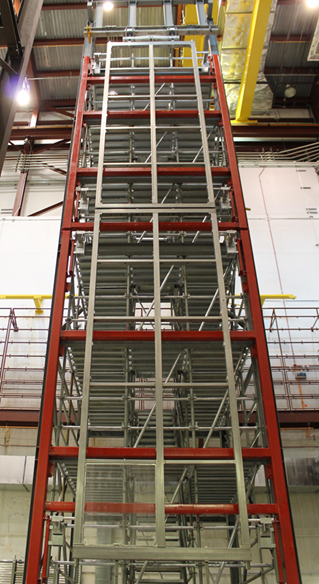
\includegraphics[height=0.5\textheight]{graphics/sp-apa-ash-river-doublet.png} 
\end{dunefigure}